% BlackboxNLP 2026 (EMNLP workshop) archival submission version.
% Anonymous review mode. Source manuscript: redundancy_dissociation.tex (unmodified).
% Style files: acl-style/acl.sty, acl-style/acl_natbib.bst (acl-org/acl-style-files).
\documentclass[11pt]{article}
\usepackage[review]{acl}
\usepackage{times}
\usepackage{latexsym}
\usepackage[T1]{fontenc}
\usepackage[utf8]{inputenc}
\usepackage{microtype}
\usepackage{amsmath,amssymb}
\usepackage{booktabs}
\usepackage{graphicx}

\title{Two Measurement Artifacts, an Unenforced Null, and What Survives in a Sparse-Autoencoder Feature-Universality Analysis}

\author{Anonymous ACL submission}

\begin{document}
\maketitle

\begin{abstract}
We report a reliability study of a natural-latent prediction for sparse-autoencoder (SAE) features: that
features which are \emph{redundant} within a model (recoverable from disjoint parts of its own
activations) are the ones that transfer across independently trained models. In building the test we
uncovered \emph{two} measurement artifacts, each of which flips or fabricates the headline. (1) On
large-activation models an unfloored ridge $R^2$ diverges to $\sim{-}1.4\times10^{5}$ for low-variance
features, producing a spurious \emph{positive} decoder-geometry correlation ($+0.27$). (2) After that is
fixed, computing the partial correlation by residualizing on \emph{raw} skewed controls (rather than on
ranks) fabricates a near-zero decoder result ($+0.001$) where the standard rank-based partial Spearman
gives $-0.12$. Third, and most instructive: the measurement plan pre-registered a \emph{position-shuffle
null} that the headline was required to beat, and our own confirmatory analysis initially failed to
enforce it. Enforcing it shows the co-firing positive does not beat the null on any pair (e.g.\ near pair
$+0.29$ observed vs.\ $+0.38$ null), and redundancy adds no detectable signal beyond it (incremental
partial $\rho$ between $-0.09$ and $+0.02$): what predicts co-firing transfer is the shuffle-invariant
\emph{context-level breadth} of a feature's activations, not redundancy structure per se. Under the single
frozen, reviewer-reproducible estimator, the surviving results are (i) a weak, consistent
\emph{negative} association between the redundancy score and decoder-geometry universality across three
model pairs ($N{=}2500$ features per pair; partial $\rho\in[-0.17,-0.12]$, all outside a permutation
null), itself largely carried by the breadth component on two pairs with a redundancy-structure-specific
negative on one pair only ($-0.23$), and (ii) a co-firing association that is real but attributable to
context breadth. We release per-feature arrays and a recompute script so every number
regenerates on a CPU in seconds. The practical lessons: within-model redundancy is not a proxy for
cross-model representational geometry; a signal that survives your permutation null can still be absorbed
by a stronger pre-registered null you forgot to run; and interpretability correlation studies are
highly sensitive to the ridge floor and the partialling convention.
\end{abstract}

\section{Introduction}
Feature universality (independently trained networks learning overlapping features) is widely reported
\citep{olah2020zoom,towards2024universality,lan2024quantifying} but lacks a predictor of \emph{which}
features transfer. Natural-latent theory \citep{wentworth2025natural} suggests one: redundant latents are
stable across ontologies, so the most redundant SAE features should be the most universal.
We set out to test this prediction and instead obtained a methodological result. Two seemingly minor choices in the
measurement pipeline, namely whether the redundancy ridge $R^2$ is floored and whether the partial
correlation is taken on raw values or ranks, each independently manufacture a different headline from the same data.
This paper documents both artifacts, freezes a single defensible estimator, and reports what survives.
The contribution is a reliability result plus a modest, honestly scoped dissociation; it is not a
universality law.

\section{Background: Natural Latents}
\label{sec:background}
Given two observable parts $X_1, X_2$ of a system and a latent $\Lambda$, natural-latent theory
\citep{wentworth2025natural} defines two conditions. \emph{Mediation:} $X_1 \perp X_2 \mid \Lambda$, so
the parts are independent given the latent and all shared structure passes through $\Lambda$.
\emph{Redundancy:} $\Lambda$ is recoverable from each part alone, $H(\Lambda \mid X_i)\approx 0$ for each
$i$. A latent satisfying both is a \emph{natural latent}, and the central theorem states that natural
latents are (approximately) isomorphic across any two agents that agree on the observable distribution:
they are the latents guaranteed to be translatable, hence universal. The theorem is from a 2025 preprint;
its guarantee is exact for the strict conditions and approximate with bounded error otherwise, and we
treat it as a motivating anchor rather than settled fact. Neither condition is a new primitive: mediation
restates conditional independence, with $\Lambda$ in the graphical role of a common cause that screens
off the parts \citep{pearl2009causality}, and redundancy is an approximate-determinism or recoverability
condition in the information-theoretic sense of \citet{cover2006elements}, distinct from the
redundant-information term of Partial Information Decomposition \citep{williams2010nonnegative}. Our
operationalization treats an SAE feature's activation as $\Lambda$ and two disjoint halves of the model's
own residual stream as $X_1, X_2$ (Section~\ref{sec:measures}); the natural-latent prediction, so
operationalized, is that highly redundant features should be the ones with cross-model matches. This
paper asks whether that prediction survives estimator scrutiny, and under which operationalization of
``universality'' it holds.

\section{Related Work}
\label{sec:related}
Natural latents were introduced by \citet{wentworth2025natural}; universality and cross-model feature
matching are studied by \citet{olah2020zoom} and \citet{towards2024universality}; SAEs by
\citet{bricken2023monosemanticity}; crosscoders and model diffing by \citet{lindsey2024crosscoders}. Most
closely related, \citet{lan2024quantifying} \emph{measure} feature-space universality across LLMs via
SAEs, \citet{thasarathan2025universal} \emph{jointly train} a single cross-model (``universal'') SAE that
aligns concepts across models, and \citet{paulo2025different} show that SAEs trained on the same data
learn different features. We differ in asking a \emph{reliability} question: whether a single-model,
training-free redundancy statistic proposed as a predictor of cross-model transfer survives scrutiny of
the estimator itself, and which operationalization of universality it actually tracks. The question of
whether independently trained models converge on shared representations is broader than SAE feature
matching: the Platonic Representation Hypothesis \citep{huh2024platonic} argues that scaling drives
models toward a shared statistical representation of reality, and representational-similarity tools such
as CKA and model stitching \citep{kornblith2019similarity} measure such convergence at the level of whole
representations rather than individual features. The mediation and redundancy conditions correspond to
conditional independence \citep{pearl2009causality} and approximate recoverability
\citep{cover2006elements} respectively; our notion of redundancy is the natural-latent
data-part-recoverability sense, distinct from decoder-cosine redundancy among SAE latents and from the
redundant-information term of Partial Information Decomposition \citep{williams2010nonnegative}.

\textbf{Reliability controls and illusions.} Our position-shuffle null belongs to the control-task
lineage of \citet{hewitt2019control}: a statistic earns its interpretation only by beating a
structure-destroying control. The interpretability-illusion literature documents what happens otherwise
\citep{bolukbasi2021illusion,makelov2023illusion}, and \citet{heap2025sparse} show automated
interpretability metrics fail to distinguish trained from random transformers, i.e.\ SAEs yield
``interpretable'' features even on randomly initialized transformers. \citet{lan2024quantifying}
already apply a random-pairing permutation null and filter trivial high-frequency token features, so
permutation nulls per se are not new here; our contribution is the stronger within-context
position-shuffle null, which our plan pre-registered but our confirmatory analysis initially failed to
run. On breadth and frequency: \citet{paulo2025different} report that the latents firing most
frequently are the ones shared across eight seed-varied SAEs, the cross-seed analogue of our
context-breadth finding, which we extend to cross-architecture transfer and sharpen by showing the
redundancy score adds nothing beyond it. By contrast, \citet{gurnee2024universal} find universal
\emph{neurons} in seed-varied GPT-2 models fire sparsely and selectively; the tension plausibly
reflects the unit (neurons vs.\ SAE latents), the statistic (raw firing rate vs.\ context breadth
under frequency controls), and the regime (same-architecture seeds vs.\ cross-architecture matching),
and resolving it is future work.

\section{Measures (Frozen)}
\label{sec:measures}
\textbf{Redundancy} (predictor, computed on model A alone). Split A's residual stream into two disjoint
halves by dimension parity; for feature $f$, $\mathrm{redundancy}(f)=\min(R^2_{L\to f}, R^2_{R\to f})$
where $R^2_{H\to f}$ is the in-sample ridge $R^2$ predicting $f$'s activation on one half from a
unit-variance PCA summary of the other half's residual, floored at $-1$. This uses no second model and no
other SAE feature, so it cannot be circular with the co-firing target.

\textbf{Universality} (targets). Features are matched across models by a third channel (token-level
max-activation correlation), then read two ways: $U_{\text{dec}}$, the aligned cross-model decoder cosine
(with a shuffled-decoder baseline); $U_{\text{overlap}}$, the Jaccard overlap of top-context sets.

\textbf{Statistic (frozen).} Partial Spearman: rank all variables, residualize $\mathrm{rank}(x)$ and
$\mathrm{rank}(y)$ on the ranked controls $\{$frequency, magnitude, decoder norm$\}$ by OLS, and take the
Pearson correlation of residuals. Each cell uses $N{=}2500$ matched features per pair. Uncertainty:
feature-bootstrap $95\%$ CI ($n{=}1000$); a permutation null ($n{=}1000$, shuffling the predictor) sets
the band a coefficient must exit to count. \emph{Declared deviation from the pre-registered plan:} the
frozen analysis plan specified bootstrap resampling over co-firing-clustered feature \emph{groups} to
respect dependence between co-firing features; the CIs reported here instead resample individual
features, which may understate interval width under co-firing dependence.

\textbf{Acceptance criteria (frozen before any blocking run).} AC1 (co-firing predictor): partial
$\rho>{+}0.20$ at $p<0.01$ on at least 2 of 3 pairs. AC2 (decoder null): partial $\rho$ in
$[-0.20,+0.10]$ on all 3 pairs with the alignment positive control passing. Cells below threshold are
reported as refuted or scoped; thresholds never move.

\section{Two Artifacts}
\label{sec:artifacts}
\textbf{Artifact 1: the ridge blow-up.} For a feature with a large mean and small residual variance,
$R^2=1-\mathrm{ss\_res}/\mathrm{ss\_tot}$ has a small denominator, so an imperfect fit yields an extreme
negative value; on Gemma/Llama-scale activations the mean redundancy $R^2$ reached $\sim{-}1.4\times10^5$.
These degenerate scores correlated spuriously, giving a decoder-geometry $\rho=+0.27$ on the near pair.
Flooring $R^2$ at $-1$ removes it; a regression test (\texttt{test\_harness\_bug.py}) fails pre-fix and
passes post-fix.

\textbf{Artifact 2: the raw-control partial.} With the floor in place, residualizing raw redundancy and
raw $U_{\text{dec}}$ on the \emph{raw} (skewed) controls before Spearman gives near-pair $\rho=+0.001$;
the standard rank-based partial Spearman on the identical arrays gives $-0.122$. The ``corrected zero''
was itself a partialling artifact. We freeze the rank-based estimator and recompute all cells with it.

\begin{figure}[t]\centering
\includegraphics[width=\columnwidth]{fig_artifacts.pdf}
\caption{The same near-pair data yields three different decoder-geometry headlines depending on two
measurement choices: an unfloored ridge (pre-fix, the historically reported $+0.27$), residualizing the
partial on raw skewed controls ($+0.001$), and the frozen rank-based partial Spearman ($-0.12$). Each
choice alone is enough to invert the conclusion.}
\label{fig:artifacts}
\end{figure}

\section{The Unenforced Null}
\label{sec:null}
The harness pre-registered a second, stronger control that the confirmatory analysis never enforced: a
\emph{position-shuffle null}. For each context, token positions are permuted independently before the
residual stream is split into halves; redundancy is then recomputed on the shuffled halves. This preserves
each feature's context-level activation profile (which contexts it fires in, and how much) while
destroying within-context positional structure, so the shuffled score isolates the \emph{context-breadth}
component of redundancy. The pre-registered standard was that the headline association must beat this
null. It does not (Table~\ref{tab:null}): on every pair the shuffled predictor associates with co-firing
universality at least as strongly as the real one ($+0.38$ vs.\ $+0.29$ near; $+0.21$ vs.\ $+0.17$;
$+0.08$ vs.\ $+0.005$), the two scores are highly rank-correlated ($\rho=0.64$--$0.86$), and the
incremental partial of redundancy given the null is indistinguishable from zero or negative for
co-firing on all pairs ($-0.09$ to $+0.02$) while the reverse partial retains signal ($+0.12$ to
$+0.26$). Feature-bootstrap $95\%$ CIs ($n{=}1000$; Block 4b of the recompute script) put uncertainty on
the load-bearing comparisons: the co-firing incremental partials span zero or are negative (near
$[-0.084,+0.014]$; Gemma $[-0.124,-0.048]$; Mistral $[-0.020,+0.051]$), and the difference
$|\text{real}|-|\text{null}|$ is \emph{negative} on all three co-firing cells (near $[-0.124,-0.058]$;
Gemma $[-0.099,-0.011]$; Mistral $[-0.072,-0.018]$): the shuffled score is a significantly
\emph{stronger} predictor than the real one. The shuffle-null column uses the single stored shuffle
realization (one independent position permutation per context, fixed at harness run time). The
shuffle-\emph{invariant} component carries the co-firing association; the shuffle-\emph{sensitive}
(position-structure) component adds nothing detectable. For decoder geometry the picture differs by
pair: on the Gemma pair the negative association \emph{strengthens} beyond the null (incremental
$-0.225$, CI $[-0.262,-0.184]$), while on the near and Mistral pairs the unique redundancy component is
small and of \emph{opposite} sign (CIs $[+0.019,+0.092]$ and $[+0.005,+0.081]$), so there the negative
is carried by the breadth component.

\begin{table}[t]\centering\small
\begin{tabular}{lcccc}
\toprule
Pair & real & null & red$\mid$null & null$\mid$red \\
\midrule
\multicolumn{5}{l}{\emph{Co-firing} ($U_{\text{overlap}}$)}\\
near & $+0.291$ & $+0.382$ & $-0.035$ & $+0.261$ \\
Gemma & $+0.005$ & $+0.081$ & $-0.086$ & $+0.118$ \\
Mistral & $+0.169$ & $+0.213$ & $+0.017$ & $+0.133$ \\
\midrule
\multicolumn{5}{l}{\emph{Decoder geometry} ($U_{\text{dec}}$)}\\
near & $-0.122$ & $-0.190$ & $+0.057$ & $-0.157$ \\
Gemma & $-0.169$ & $-0.029$ & $-0.225$ & $+0.153$ \\
Mistral & $-0.159$ & $-0.253$ & $+0.044$ & $-0.204$ \\
\bottomrule
\end{tabular}
\caption{Position-shuffle null (same frozen partial-Spearman estimator and controls). ``real'' is the
observed partial $\rho$; ``null'' uses the position-shuffled redundancy score (single stored
realization); the last two columns are incremental partials of each predictor given the other. The
co-firing headline never beats the null and retains no unique signal beyond it: feature-bootstrap
$95\%$ CIs ($n{=}1000$) on $|\text{real}|-|\text{null}|$ are negative on all three co-firing cells
(Section~\ref{sec:null}).}
\label{tab:null}
\end{table}

\section{What Survives}
\label{sec:survives}
\begin{table*}[t]\centering
\begin{tabular}{lcccc}
\toprule
Model pair & $U_{\text{dec}}$ $\rho$ & 95\% CI & $U_{\text{overlap}}$ $\rho$ & 95\% CI \\
\midrule
GPT-2 / Pythia (near) & $-0.122$ & $[-0.163,-0.081]$ & $+0.291$ & $[+0.250,+0.331]$ \\
Gemma-2-9b / Llama-3.1-8B (far) & $-0.169$ & $[-0.208,-0.128]$ & $+0.005$ & $[-0.033,+0.047]$ \\
Mistral-7B / Llama-3.1-8B (far) & $-0.159$ & $[-0.200,-0.119]$ & $+0.169$ & $[+0.130,+0.209]$ \\
\bottomrule
\end{tabular}
\caption{Frozen rank-based partial Spearman (controls: frequency, magnitude, decoder norm), $N{=}2500$
features per pair, permutation null $n{=}1000$. Every $U_{\text{dec}}$ cell and both non-null
$U_{\text{overlap}}$ cells lie outside their per-cell permutation bands (all bands within
$\pm0.043$; $p=0.001$); the Gemma
$U_{\text{overlap}}$ cell is inside it ($p=0.836$). Only the near-pair $U_{\text{overlap}}$ cell clears
the pre-registered AC1 threshold of $+0.20$; the Mistral cell ($+0.169$) is outside the null but below
threshold.}
\label{tab:main}
\end{table*}

\begin{figure}[t]\centering
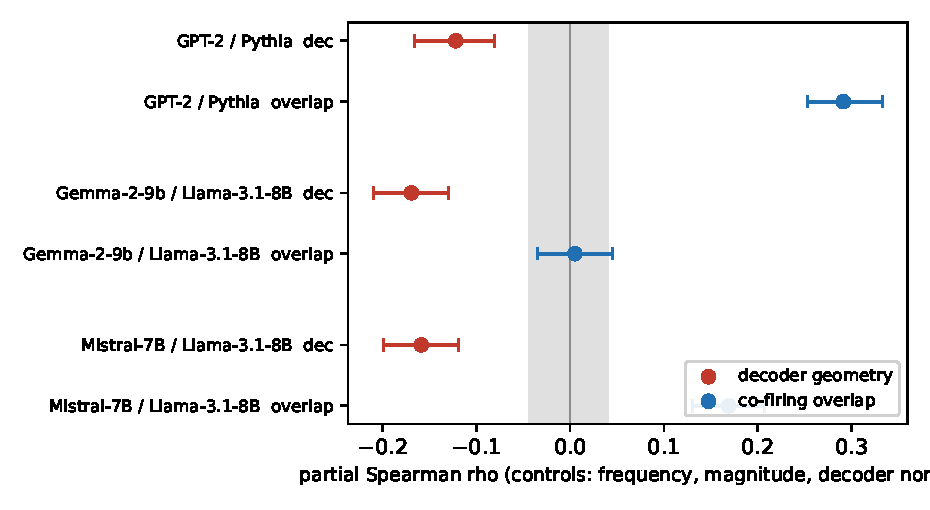
\includegraphics[width=\columnwidth]{fig_forest.pdf}
\caption{The dissociation at a glance. Partial Spearman rho (95\% feature-bootstrap CI) of redundancy
against each universality measure, across the three pairs; grey band is the permutation null. Every
decoder-geometry point (red) is a small negative outside the null; the co-firing points (blue) are
positive on the near and Mistral pairs (only the near pair clears the pre-registered $+0.20$ threshold)
and null on the Gemma pair. Sign depends on which universality is measured.}
\label{fig:forest}
\end{figure}

\begin{figure*}[t]\centering
\includegraphics[width=0.92\textwidth]{fig_scatter.pdf}
\caption{Near-pair (GPT-2/Pythia) rank-residualized scatter: redundancy is weakly \emph{negatively}
related to decoder-geometry universality (left) yet \emph{positively} related to co-firing universality
(right), on the same features.}
\label{fig:scatter}
\end{figure*}

\textbf{Decoder geometry: a small, consistent negative, neither zero nor the prior positive.} Across all
three pairs redundancy is weakly \emph{anti}-associated with decoder-cosine universality
($\rho\in[-0.17,-0.12]$, $1.5$--$2.9\%$ variance), every CI excluding zero on the negative side, every
coefficient outside the permutation null (Table~\ref{tab:main}, Figure~\ref{fig:forest}). The measure itself is informative (it exceeds its shuffled-decoder baseline in every run), so this is a genuine weak negative rather than an artifact of an insensitive measure. Against the position-shuffle null the negative is largely carried by the context-breadth
component on two pairs, but on the Gemma pair the position-structure component contributes an additional
negative beyond the null ($-0.225$, Table~\ref{tab:null}).

\textbf{Co-firing: real association, but carried by context breadth, and confirmed on 1 of 3 pairs under
the frozen criterion.} Redundancy is positively associated with co-firing universality on the near pair
($+0.291$) and one far pair ($+0.169$), both outside the permutation null, but not the other far pair
($+0.005$, inside the null). The pre-registered acceptance criterion AC1 required partial $\rho>{+}0.20$
on at least 2 of 3 pairs; only the near pair clears $+0.20$, so \emph{AC1 is not met} (1 of 3 pairs).
More decisively, Section~\ref{sec:null} shows the association
never beats the pre-registered position-shuffle null and retains no unique signal beyond it, so the
surviving claim is that a feature's \emph{context-level activation breadth} predicts co-firing transfer;
\emph{redundancy structure adds nothing detectable}. An earlier pilot estimate of the near-pair
co-firing association ($+0.41$) was non-confirmatory and is superseded by the frozen gate-3 recomputation
reported here. Because redundancy is defined on model A's residual stream alone, the association that
does appear is not a co-firing tautology.

\textbf{The dissociation.} On the same features and score, redundancy's relationship to universality has
opposite sign under the two universality operationalizations: mildly negative for decoder geometry on all
three pairs, positive where present for co-firing, with the co-firing side attributable to context
breadth rather than redundancy structure (Figure~\ref{fig:scatter}, Table~\ref{tab:null}). Which
``universality'' you measure decides the answer, and which null you enforce decides the mechanism you may
claim.

\section{Discussion}
\label{sec:discussion}
The natural-latent prediction, read as a claim about representational geometry, is falsified in a mild
direction here: more-redundant features are, if anything, slightly \emph{less} likely to have an aligned
decoder in a second model. The co-firing association is real but, once the pre-registered
position-shuffle null is enforced, it is attributable to context-level activation breadth rather than to
redundancy structure; behavioral overlap and geometric alignment come apart either way. For
practitioners: do not use within-model redundancy as a cross-model transfer screen, particularly for
representation geometry, and treat breadth of firing as the default confounder to rule out in
transfer-prediction claims. For methodology, three lessons with the same shape: an unfloored ridge and a
raw-control partial are each sufficient to invert a headline, and a pre-registered null that goes
unenforced can silently upgrade ``context breadth predicts transfer'' into ``redundancy predicts
transfer.'' Correlation-over-features interpretability studies should pre-register the estimator, run
\emph{every} registered null, and release the per-feature arrays.

\section*{Limitations}
Three pairs only, one layer each (a multi-layer robustness sweep and a third non-Llama-anchored far pair
are the two open blocking runs), so generality beyond these pairs is unestablished. Each model is
represented by a single publicly released SAE; SAE training is itself unstable across seeds
\citep{paulo2025different}, so SAE-level variance is unmeasured here. The co-firing universality measure
presupposes that the cross-model feature matching (token-level max-activation correlation) is meaningful;
if the matching is poor or picks up superficial co-activation, the co-firing target inherits that
weakness. The co-firing measure may also retain co-activation base-rate structure beyond the frequency
control. We do not resolve why the Gemma co-firing cell is null while Mistral is positive. The reported
bootstrap CIs deviate from the pre-registered group-level resampling scheme (Section~\ref{sec:measures})
and may be anti-conservative.
The redundancy predictor is an in-sample ridge $R^2$ on a PCA summary, an operational proxy for the
theoretical recoverability condition $H(\Lambda \mid X_i)\approx 0$ rather than the full quantity, so a
null or negative here bounds the proxy, not the theorem, whose guarantee requires mediation and
redundancy jointly. The position-shuffle null itself preserves context-level co-occurrence, so our
attribution of the co-firing signal to ``context breadth'' is an interpretation of what survives the
shuffle, made post hoc once the unenforced null was discovered, not a pre-registered mechanism claim.
All findings are correlational; no causal claim is made. The two artifacts we
document are specific to ridge-$R^2$ redundancy scores and OLS-residualized partial correlations; other
estimator families may harbor analogous failure modes we do not survey.

\section*{Ethics Statement}
This work uses only publicly released pretrained language models (GPT-2, Pythia, Gemma-2-9b,
Llama-3.1-8B, Mistral-7B) and their publicly released sparse autoencoders, together with public corpora.
It involves no human subjects, no private or personally identifying data, and no release of any new model
weights. The results require no training and regenerate from released per-feature arrays on a CPU. We
note a safety-relevant implication: predictors of which interpretability findings transfer across models
bear on the argument that auditing a small model informs claims about a larger one; our results caution
that such predictors can be artifacts of the estimator, so transfer claims should be accompanied by
frozen, reproducible measurement pipelines.

\section*{Reproducibility Statement}
Contracts (measures, analysis plan, both artifacts) are frozen at git commit \texttt{37a266f} of the
anonymized repository. Every number regenerates from the released per-feature arrays via
\texttt{recompute\_partials.py} on a CPU in seconds, including the position-shuffle-null and
incremental-partial analysis of Section~\ref{sec:null} (Block 4 of the script). The harness $R^2$ floor is covered by a regression
test (\texttt{test\_harness\_bug.py}) that fails pre-fix and passes post-fix. Pre-correction values
appear only as labeled artifacts, and pilot point estimates (including the near-pair co-firing $+0.41$)
were labeled non-confirmatory at freeze time and are superseded by the frozen gate-3 recomputation. Data availability: the per-feature arrays are included in the
supplementary material / anonymous repository (link redacted for review).

\bibliography{bbnlp}

\appendix
\section{Experimental Setup}
\label{app:setup}
All activations come from $3000$ contexts of $64$ tokens drawn from a public Pile sample
(\texttt{NeelNanda/pile-10k}), streamed identically for both models of a pair. Models and SAEs (all
publicly released, via \texttt{sae\_lens} / \texttt{transformer\_lens}): \textbf{near pair} GPT-2-small,
layer-8 residual post (\texttt{gpt2-small-resid-post-v5-32k}) vs.\ Pythia-70m-deduped, layer-4 residual
post (\texttt{pythia-70m-deduped-res-sm}); \textbf{Gemma pair} Gemma-2-9b-it, layer-20 residual post,
width 16k canonical (\texttt{gemma-scope-9b-it-res-canonical}) vs.\ Llama-3.1-8B-Instruct, layer-16
residual post, Llama-Scope $8\times$ (\texttt{llama\_scope\_lxr\_8x}, \texttt{l16r\_8x}); \textbf{Mistral
pair} Mistral-7B, layer-16 residual pre (\texttt{mistral-7b-res-wg}) vs.\ the same Llama-3.1-8B SAE.
Per pair, the $N{=}2500$ most active model-A features are scored. Redundancy:
$\min(R^2_{L\to f}, R^2_{R\to f})$, where each $R^2$ is an in-sample closed-form ridge fit
($\lambda{=}1$) predicting the feature's per-context half-mean activation from a $48$-dimensional PCA
summary of the \emph{opposite} residual-stream half (halves by dimension parity), floored at $-1$.
Cross-model matching: token-level max-activation correlation; $U_{\text{overlap}}$ is the Jaccard
overlap of top-$50$ context sets; $U_{\text{dec}}$ is the aligned cross-model decoder cosine with a
shuffled-decoder baseline. The position-shuffle null permutes token positions independently per context
before the half split (one stored realization). Bootstrap and permutation sizes are $n{=}1000$
throughout. The released arrays contain, per feature: redundancy (real and position-shuffled), both
universality scores, frequency, magnitude, and decoder norm.

\end{document}
